\documentclass{article}
\usepackage{geometry}
\usepackage[english]{babel}
\usepackage[utf8]{inputenc}
\usepackage{fancyhdr}
\usepackage{graphicx}
\usepackage{titlesec}


\setlength{\headheight}{15.2pt}
\setcounter{secnumdepth}{3}
\rfoot{Pg: \thepage}

\geometry{
   a4paper,
   left = 20mm,
   top = 20mm,
}
\begin{document}
\thispagestyle{empty}

\section*{}
{\LARGE\makebox[\textwidth]{\textbf{KATHMANDU UNIVERSITY}}}

\centerline{Department of Computer Science and Engineering}
\centerline{Dhulikhel,Kavre}
\begin{figure}[h]
    \centerline{
\includegraphics[width=50.546mm,height=50.546mm]{KU_Logo.png}}
\end{figure}

\centerline{\textbf{A Project Proposal}}
\centerline{on}
\centerline{\underline{\textbf{"Covid-19 Situation Analysis Application"}}}

\vspace*{12mm}

\centerline{\textbf{[Code No. : COMP 206]}}
\centerline{(For partial fulfillment of 2nd Year/ 3rd Semester in Computer Science)}

\vspace*{10mm}

\centerline{\textbf{Submitted by}}
\centerline{\textbf{Aayush Pokharel(Roll No. 43)}}
\centerline{\textbf{Dikshya Poudel (Roll No. 45)}}
\centerline{\textbf{Sajag Pradhanang (Roll No. 47)}}
\centerline{\textbf{Samjhana Bhusal (Roll No. 60)}}

\vspace*{16mm}


\centerline{\textbf{Submitted to}}
\centerline{\underline{\textbf{Project Cordinator}}}
\centerline{\textbf{Nabin Ghimire}}
\centerline{\textbf{Dept of Computer Science and Engineering}}

\vspace*{10mm}

\centerline{\textbf{Submission Date: 23th June, 2021}}



\clearpage
\thispagestyle{empty}

\section*{Abstract}
The project ‘Covid-19 Situation Analysis Application’ proposal is drafted to meet the prerequisites to partially fulfill the COMP 206 course offered by the 
Department of Computer Science and Engineering at Kathmandu University and to cover for the pitfall of previously proposed Project ‘Portfolio Management and 
Finance Management Application’ . This project is designed to overcome the lack of centralized facility to deeply analyse COVID-19 situational data on international 
and national level. We, the involved project members, have decided to create a compact application that can run on Windows platform which scrapes data from multiple sites 
like worldometer.info, mohp.gov.np, covidnepal.org, covid19.wh.int and kaggle.com  allowing us to work on the dataset and plot various diagrams and charts necessary for in 
depth demographic analysis. It will allow customizing the charts based on demographic factors like age sex, population density, country etc and also present trends before, 
during and after a major wave. We are accomplishing this project by using dynamically typed object oriented programming language(Python) and Qt framework to handle the GUI 
portion of the application, Selenium and Scrapy to scrape web data, pandas for handling dataset and matplotlib and QTGraph to finally plot the data. The main goal of this 
project is to develop an efficient set of python code that can stand up to real world scenarios while increasing the programming skill of involved project members in hope 
of tackling harder projects in the forthcoming days.

\clearpage
\thispagestyle{empty}
\tableofcontents

\clearpage
\thispagestyle{empty}
\listoffigures

\clearpage
\pagenumbering{arabic}
\section{CHAPTER 1: INTRODUCTION}

\subsection{Background}
COVID-19 pandemic is a global problem. It has stifled the global economy, caused untold amounts of grief among family members and friends, forced people into social 
distancing and lockdown as means of virus transmission prevention.
\\\\
Compared to some other countries, Nepal was still in a better situation during the first wave of the pandemic but during the second wave was hit quite worse.
\\\\
There are few available sites that publish information on the covid situation but any data required for an in depth analysis based on different demographic factors 
are needed to be sourced from different websites. The lack of standardization of data between different websites causes cross referencing to be very difficult. To 
challenge this difficulty, we are aiming to make an open source program that is available to everyone with no cost overhead for operation. This system will be used 
by end users for the purpose of analyzing the COVID-19 situation on an international as well as on national level based on various demographics
\\\\
Furthermore, this application shall also report on the availability of medical infrastructures available in Nepal to COVID-19 patients based on geographical region.

\vspace*{5mm}
\subsection{Onjectives}
The main objective of this project is to understand the intermediate concepts of dynamically typed language and web scraping for enhancing our knowledge to solve 
real life problems using an Object-oriented paradigm. Besides, the other objectives are listed below:
\begin{itemize}
    \item To make various configurable graphs of multiple demographic indicators to facilitate technical analysis.
    \item To make an app which can keep people updated about the COVID-19 situation at local,national and international level. 
    \item To create a database that allows user to know about the current medical facilities near them.     
\end{itemize}

\vspace*{5mm}
\subsection{Motivation and Significance}
Our project is particularly inspired by various sites like Worldometer and covid19.mohp.gov.np. This program is being designed with an aim of collecting data that 
are available on those sites with our prior experience of the struggle of getting information in an intuitive manner.. This will present a relevant user interface 
which provides easy, enjoyable and effective interaction between the user and the application along with the explanation of various graphs and their trends. Most 
notably, it will allow for analysis of transmission and mortality trends with cross reference to health infrastructures via line graph, making it more accessible 
for in depth understanding of the pandemic situation to a person untrained in technical analysis. Furthermore, this program presents features such as Vaccine 
development situations, local governmental updates, etc to facilitate understanding about the pandemic among users as a means to combat its spread.

\clearpage

\section{RELATED WORKS}
There are similar sites available which are being used globally as well as nationally which are being operated by different NGO and governmental organizations and 
to keep track of the COVID-19 pandemic.
\\\\
Some of such sites that are in use are:

\subsection{worldometer.org}
\begin{figure}[h]
    \centerline{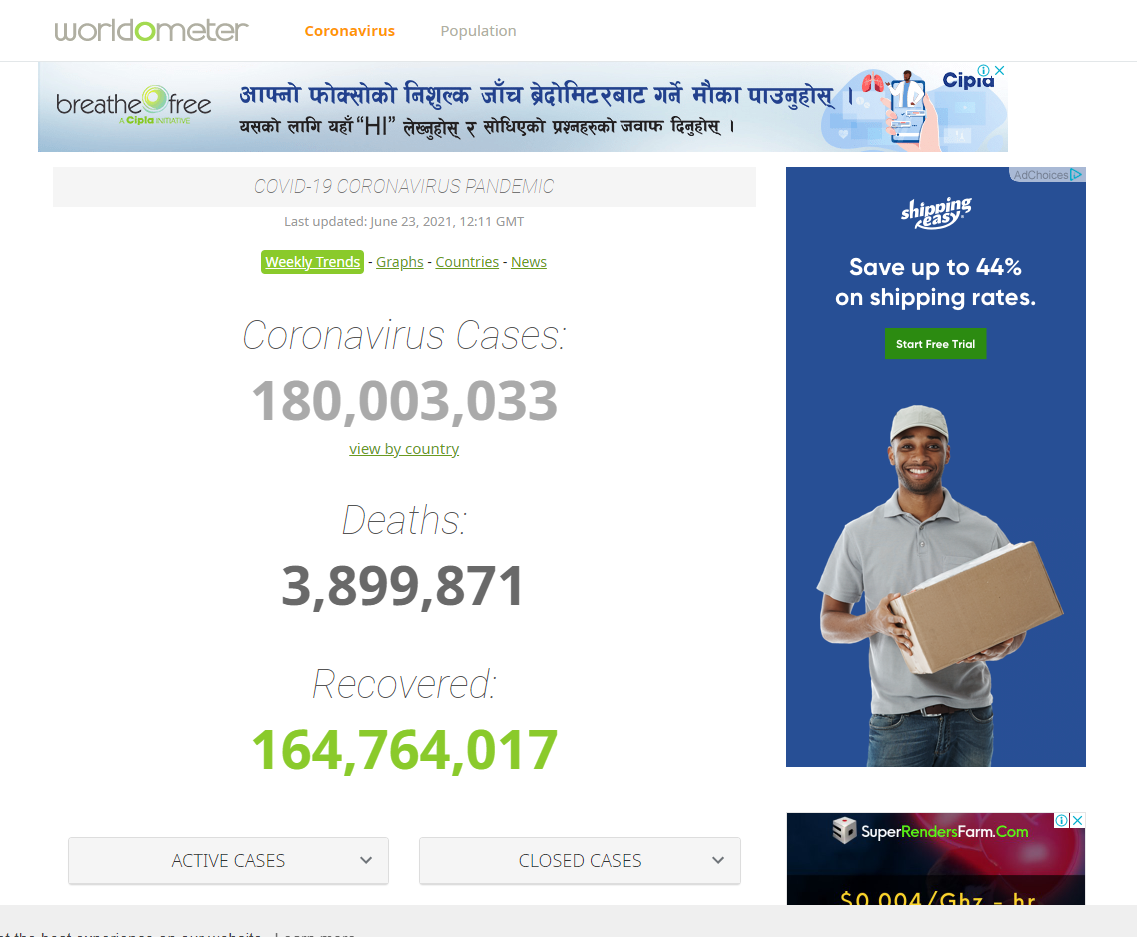
\includegraphics[width = 50mm]{worldometer.png}}
    \caption{Worldometer Website}
    \label{fig}
\end{figure}


\subsection{covid19.mohp.gov.np}
\begin{figure}[h]
    \centerline{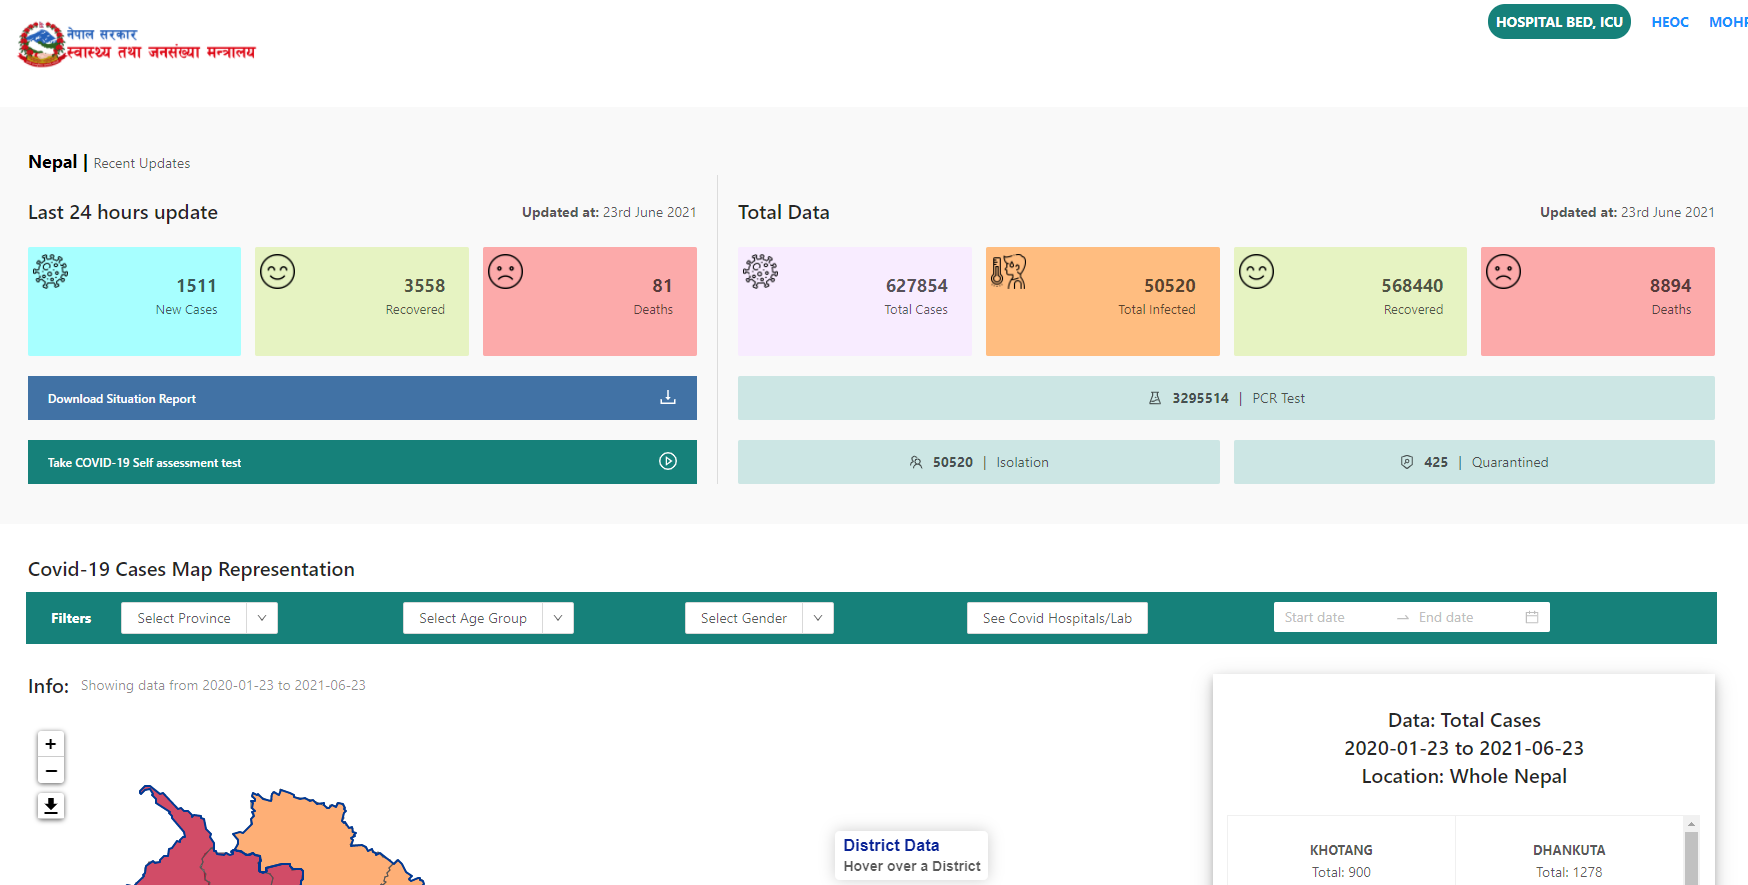
\includegraphics[width = 50mm]{mohp.png}}
    \caption{Ministry of Health and Population Website}
    \label{fig}
\end{figure}


\subsection{covidnepal.org}
\begin{figure}[h]
    \centerline{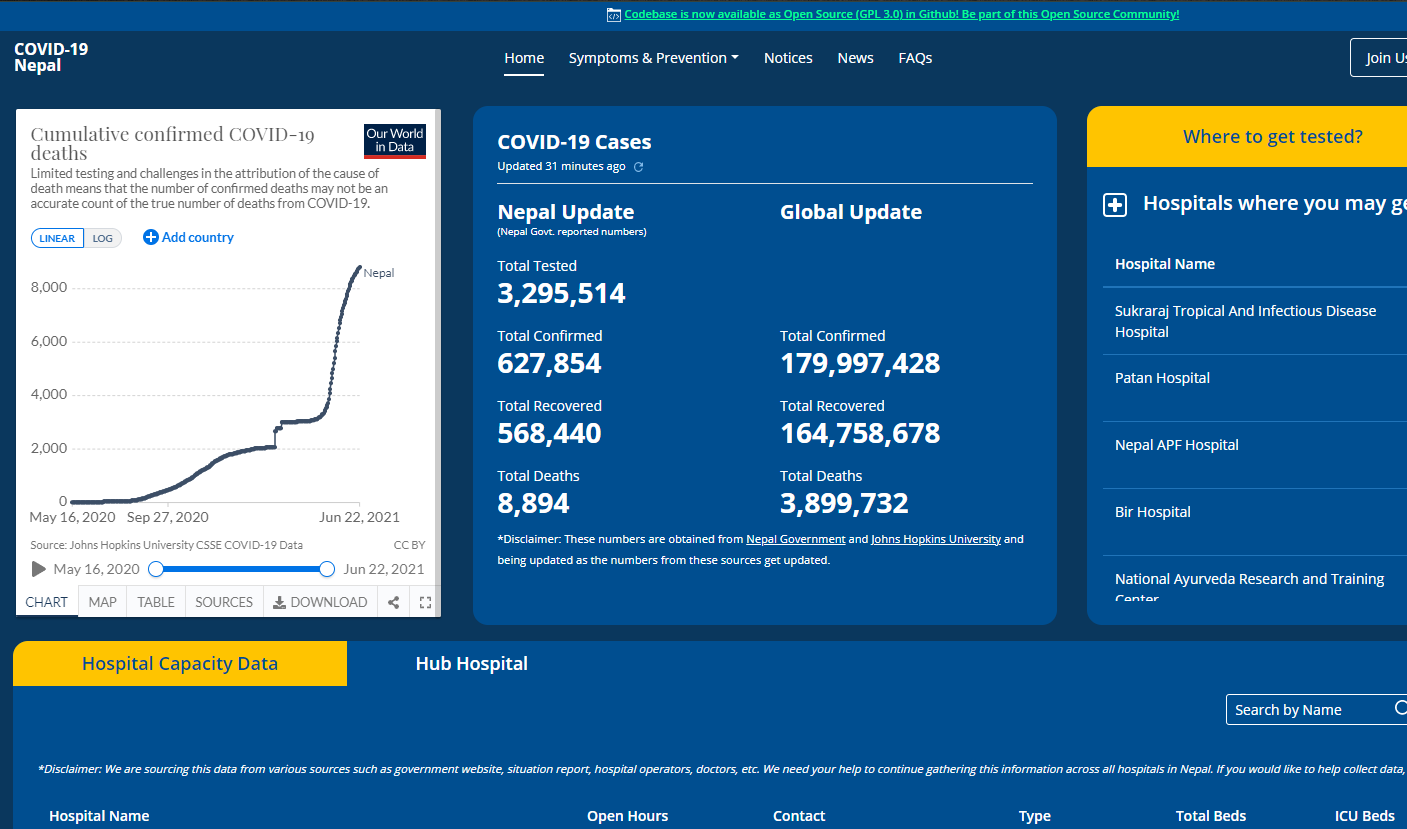
\includegraphics[width = 50mm]{covidnepal.png}}
    \caption{CovidNepal.org Website}
    \label{fig}
\end{figure}


\clearpage

\section{CHAPTER 3: PROCEDURE AND METHODS}
The whole process of developing the software has been divided into following aspects:
\begin{itemize}
    \item Research and study
    \item UI Design and prototyping
    \item Core programming
    \item Program Testing
    \item Documentation
\end{itemize}

\subsection{Research and Study}
This project being the first of the kind we have ever done, we decide to choose a subject matter that we clearly know and have experience with ie. the plotting graph 
using matplotlib and database handling. We have interacted with the various software/sites mentioned above on a semi-regular basis and have experienced its strength 
and pitfall. While clearly not being as extensive and feature rich as the software/sites available in the market today,we are trying to overcome the paywall  that 
we have experienced while using these software/sites to conduct technical analysis. So our project will mainly focus on various financial indicators, their graphs, 
share calculator and portfolio management.

\subsection{UI design and Prototyping}
The initial designs are sketched on A4 papers by our members and shared on group chat for peer review and then use QT Creator’s design tab to stub test the look 
of our UI before adding any functionality to the various widgets.

\subsection{Core Programming}
The most amount of project time is going to be spent in this stage. We are using the Python language to write our program. QT framework provides the necessary 
tools to create the GUI. Selenium is being used to surf the web and get html of webpages and scrapy is being used on the html file to parse and extract data 
which is converted into datasets via Pandas for easy import and manipulation as per end user requirement; for instance, getting data of certain dates only. 
Finally the QTGraph and matplotlib library is used to plot the dataset.

\subsection{Program Testing}
Unit testing is done as soon as we complete the code of a single widget to check its functioning properly. This is repeated multiple times during the development 
period to create a robust system and once the core programming is completed, alpha testing is done to find different types of bugs or ill optimised issues.

\subsection{Documentation}
A document containing all the features and functions of the programs will be listed along with their use case after all the testing is completed and the program 
is ready to be published.


\clearpage

\section{CHAPTER 4: SYSTEM REQUIREMENTS AND SPECIFICATIONS}

\subsection{Software Requirements:}
\vspace*{5mm}
\subsubsection{Front End Tools}
\begin{itemize}
    \item The program is created using Python.
    \item Development Tools : QT frameworks    
\end{itemize}
\subsubsection{Back End Tools}
\begin{itemize}
    \item Selenium and Scrapy modules used for scraping web information.
    \item Pandas module used to make datasets.
    \item Matplotlib and QTGrapgh used for plotting.
\end{itemize}
\subsection{Hardware Requirements:}
\begin{itemize}
    \item Compatibility: Compatible with all PCs running on Windows platform.
\end{itemize}

\vspace*{20mm}
\paragraph{Python :} A dynamically typed multi paradigm general purpose programming language.
\paragraph{QT frameworks :} An open source cross platform multi language widget toolkit that helps in developing GUI Application.

\clearpage

\section{CHAPTER 5: PROJECT PLANING AND SCHEDULING}
\begin{figure}[h]
    \centerline{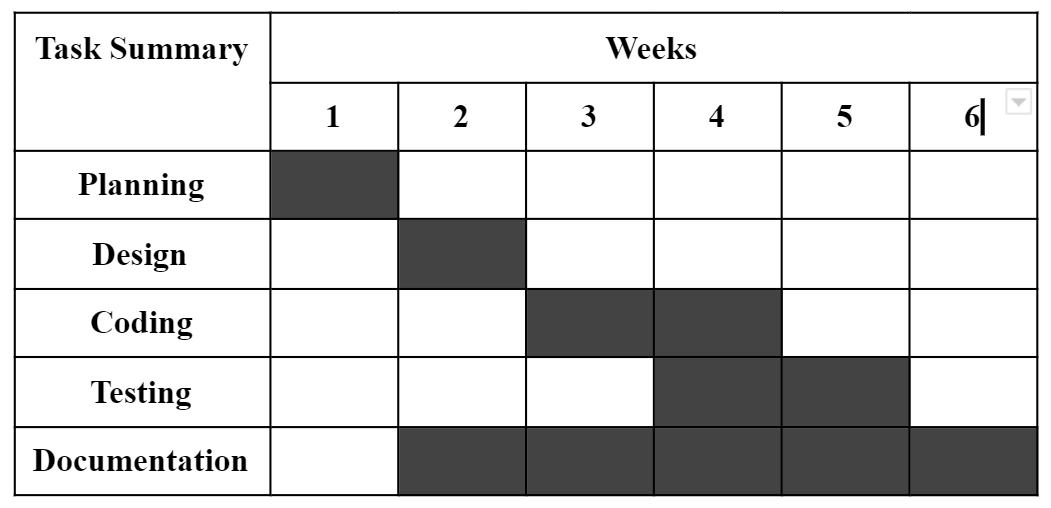
\includegraphics[width = 190mm]{chart.png}}
    \caption{Gant Chart}
    \label{fig}
\end{figure}

\rightline{\underline{\textbf{Index}}}
\begin{figure}[h]
    \rightline{
\includegraphics[width=15mm,height=15mm]{box.png}}
\end{figure}
\rightline{\underline{\textbf{Task Completed}}}

\clearpage

\section{Refrences}
\end{document}